\documentclass[12pt,twocolumn]{article}
\usepackage[margin=1.5cm]{geometry}
\usepackage{amsmath}
\usepackage{graphicx}
\usepackage{hyperref}
\title{Properties of Concave Lenses}
\author{Prof. Jordan C. Hanson}

\begin{document}
\small
\maketitle

\section{Introduction}

\noindent
In this activity, we will verify the \textit{thin lens equations}:

\begin{align}
\frac{1}{d_{\rm o}} + \frac{1}{d_{\rm i}} =& \frac{1}{f} \label{eq:f} \\
m = \frac{h_{\rm i}}{h_{\rm o}} =& -\frac{d_{\rm i}}{d_{\rm o}}  \label{eq:m}
\end{align}

In Eq. \ref{eq:f}, $d_{\rm o}$ is the distance between the object and the lens origin, and $d_{\rm i}$ is the distance to the image.  In this lab activity, we will use a concave lens with a focal length $f$ that produces real images.  The parameter $m$ is called the magnification, representing the ratio of image height $h_{\rm i}$ to object height $h_{\rm o}$.

We will verify Eq. \ref{eq:f} by varying $d_{\rm o}$ with respect to the lens origin and measuring $d_{\rm i}$.  The value of $d_{\rm i}$ corresponds to the distance from lens origin at which the real image is in focus. The focal length $f$ is a constant in this experiment.  Thus, the only measurement required to verify Eq. \ref{eq:f} is $d_{\rm i}$.  To verify Eq. \ref{eq:m}, we will confirm two facts.  First, we will confirm that the focused image is inverted and that $d_{\rm i}>0$, which will justify the minus sign in Eq. \ref{eq:m}.  Second, we will measure $m$ geometrically, and verify that this matches $d_{\rm i}/d_{\rm o}$.

\section{Experimental Setup}

\begin{figure}[ht]
\centering
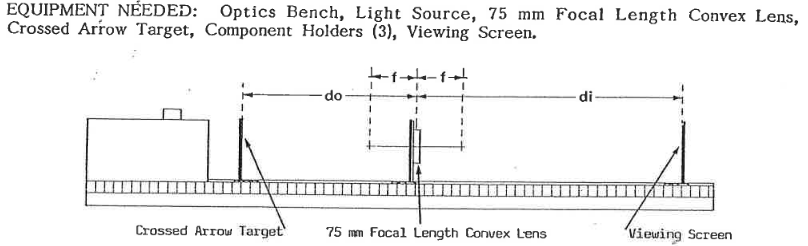
\includegraphics[width=0.49\textwidth,trim=0cm 0cm 0cm 2cm,clip=true]{equip.png}
\caption{\label{fig:equip} A diagram of the setup.}
\end{figure}

\noindent
The procedure depicted in Fig. \ref{fig:equip} should produce results that verify Eqs. \ref{eq:f} and \ref{eq:m}.  Check that you have the following items at your table:

\begin{itemize}
\item Optics bench
\item Light source
\item Magnetic object holder with crossed-arrow target
\item Magnetic object holder with concave lens ($f = 75$ mm or $f=150$ mm)
\item Magnetic object holder with viewing screen
\item Meter stick
\end{itemize}

Place the light source as far as possible at one end of the optics bench.  Plus the crossed arrow target in front of the light source using the magnetic holder.  Using another magnetic holder, place the concave lens more than one focal length away from the target.  The designed focal length is written on the lens, and we will verify this constant with our measurements.  Finally, place the viewing screen more than one focal length from the lens origin, using a magnetic holder.  Plug in the light source, and turn it on.  Adjust the primary ray direction with the knob on the top of the light source as necessary.  Move the viewing screen forwards and backwards until a focused image forms on it.

%\section{Data and Error Analysis}
%
%\noindent
%Activate the light source.  The light should pass through be emitted through the slits as a ray-like source with vertical extent.  The ray should project onto the ray table along the normal direction, marked with 0 degrees.  The ray should exit the cylindrical lens, and continue along the normal direction marked with 0 degrees.  If there is a slight misalignment, make a small adjustment using the knob on top of the light source.  The knob rotates the slight source by a few degrees, which helps ensure that 0 degrees into the lens corresponds to 0 degrees coming out of the lens.
%
%As you rotate the ray table, add $\theta_2$ data to Tab. \ref{tab:data}.  We have set 0 degrees in to correspond to 0 degrees out, so we do not need to measure this.  Use Eq. \ref{eq:sn2} to calculate $n_2$.  The fact that the observed $n_2$ value is constant shows that Eq. \ref{eq:sn2} holds.
%
%\begin{table}[ht]
%\footnotesize
%\centering
%\begin{tabular}{| c | c | c | c |}
%\hline
%\textbf{$\theta_1$} [deg] & \textbf{$\theta_2$} [deg] & \textbf{$n_2 = \sin\theta_2/\sin\theta_1$} & \textbf{$\sigma_{n,2}$} \\ \hline
%5 & & & \\ \hline
%10 & & & \\ \hline
%15 & & & \\ \hline
%20 & & & \\ \hline
%25 & & & \\ \hline
%30 & & & \\ \hline
%35 & & & \\ \hline
%40 & & & \\ \hline
%45 & & & \\ \hline
%50 & & & \\ \hline
%55 & & & \\ \hline
%60 & & & \\ \hline
%65 & & & \\ \hline
%70 & & & \\ \hline
%75 & & & \\ \hline \hline
%\textbf{Average:} & --- & & \\ \hline
%\end{tabular}
%\caption{\label{tab:data} Perform the necessary measurements to complete this table.}
%\end{table}
%
%The error propagation formula for $n_2$ is
%
%\begin{equation}
%\frac{\sigma_{n,2}}{n_2} = \sqrt{\frac{\sigma_{\theta,1}^2}{\tan^2\theta_1} + \frac{\sigma_{\theta,2}^2}{\tan^2\theta_2}} \label{eq:err}
%\end{equation}
%
%Using Excel or Google sheets at your table, compute the error in $n_2$ using Eq. \ref{eq:err}.  The values for $\sigma_{\theta,1}$ and $\sigma_{\theta,2}$ are your decision based on the precision you perceive on the ray table.  Typical values are between 0.5 to 1.5 degrees, driven by the thickness of the light ray relative to the degree markings.
%
%\section{Graphing the Data}
%
%Did we just \textit{assume} Eq. \ref{eq:sn2} to be true, and then compute $n_2$ values based on this assumption?  If Eq. \ref{eq:sn2} does not hold, then our $n_2$ values would not be clustered tightly around the true constant value.  As a check, try graphing $\sin\theta_1$ versus $\sin\theta_2$.  The slope should be $n_2$, consistent with your value in Tab. \ref{tab:data}.  \textbf{Include a drawn version of your graph below.}

\end{document}